\chapter{IoT Security engineering}
\label{chap:iot_security}

This Chapter treats IoT security from an industrial engineering perspective. At this point of the internship, it was decided to cut the research work off, and turn more towards practical subjects. This marks the end of \emph{Stage 1} and the start of \emph{Stage 2}.

\section{Threats landscape in the IoT}

\subsection{Main threats}

As for all information systems, one of the most common threats IoT devices are facing is malware. In difference with usual malware we deal with on computer systems, IoT malwares are very often cross-architecture, because IoT devices themselves are based on different physical and processor architectures. That’s to say that antagonists are adapting their malicious payloads to the heterogeneity in IoT. Besides the damage a malware can inflict on the system by definition, the cross-architecture side of IoT malwares make them very difficult to detect and classify. Moreover, energy-constrained devices are not likely to support complex malicious code detection systems. Alhanahnah et al. [8] made a step towards proposing a signature generation for cross-architecture IoT malwares. However, the IoT malware detection problem remains very much unsolved yet.

With over 40 billions connected objects reached by 2025, IoT devices are a very seductive tool for botnets and DDoS attacks. Going back to what has just been evoked, since some IoT devices can be easily infected with malwares in a stealthy fashion, a hacker or a hackers group can then seek to infect a large numbers of objects in order to build a botnet. IoT botnets can be used to compromise heavily secured computer systems using their powerful brute-force potential. They can also be used to conduct some of the most massive DDoS attacks, such as the Dyn attack on major DNS providers carried out by the Mirai botnet in 2016 [3]. The Dyn attack was the largest DDoS attack ever seen at its time with an unprecedented flood of 1 Tbps targeting OVH servers. Its record has only been broken by the attack on AWS servers in June 2020, with a record charge of 2.3 Tbps [11]. Once again, the attack was carried out by an IoT botnet. The exponential growth of IoT connected objects is only democratising these kind of lethal attacks, and posing more serious security challenges in IoT networks security. Molesky and Cameron [9] proposed a solution based on the “White Worm” technology, which uses the very technical basis of this threat and turn it up into an asset used for benign purposes. The scheme remains pretty theoretical though, and a lot is yet to be done to bring the concept into a realistic application.

Another major threat in IoT is data privacy, and this concerns some of the most common IoT applications. For example, IoT connected objects are more and more used in healthcare and smart homes. In those kind of applications, we usually have wireless sensors and other types of objects gathering and processing intimate (eg. smart homes) and sensitive (eg. healthcare) data about individual’s. Therefore, IoT communications are a top priority target for network attacks, generally conducted by actors seeking to compromise either the confidentiality or the integrity of the transmitted data.

\subsection{IoT Malwares}

\subsubsection{BashLite}

IoT DDoS malware which comes with a C\&C \cite{securityintelligence}. Most BASHLIFE attacks are simple UDP, TCP floods and HTTP attacks. BASHLIFE infect a IoT device by brute-forcing its telnet access using known default credentials. One interesting aspect of BASHLIFE is that malware payload deployed in IoT devices has the BASHLIFE's C2s IP addresses hard-coded into it and are easier to monitor. Most of the infected devices are located in Taiwan, Brazil and Columbia. The source code of BASHLIFE was partly leaked in early 2015 and has led to many variants. BASHLIFE is considered the predecessor of Mirai and is in direct competition for vulnerable IoT real estate.

BASHLIFE/Lizkebab/Torlus/gafgyt is one of the popular malware which infects Linux based IoT devices to launch DDoS attacks. It was reported that BASHLIFE is responsible for enslaving over 1 million IoT devices, constituting mostly of Internet enabled cameras and DVRs. It is capable of launching attack of up to 400 Gpbs. Most BASHLIFE attacks are simple UDP, TCP floods and HTTP attacks. BASHLIFE infect a IoT device by brute-forcing its telnet access using known default credentials. One interesting aspect of BASHLIFE is that malware payload deployed in IoT devices has the BASHLIFE's C2s IP addresses hard-coded into it and are easier to monitor. Most of the infected devices are located in Taiwan, Brazil and Columbia. The source code of BASHLIFE was partly leaked in early 2015 and has led to many variants. BASHLIFE is considered the predecessor of Mirai and is in direct competition for vulnerable IoT real estate.

\subsubsection{BusyBotNet}

This IoT malware comes with embedded tools usually found on full systems dedicated for ethical hacking. These toolset include Hydra, masscan, tshark and reverse shell backdoors.

\subsubsection{Lightaidra}

LightAidra/Aidra is a IRC-based mass scanning and exploitation tool support on several architectures, namely MIPS, MIPSSEL, ARM, PPC, x86/86-64 and SuperH. Malware is designed to search open telnet ports that could be accessed using known default credentials. The source code of LightAidra is freely available on the Internet as open source project. It allows scanning and exploiting routers for make BOTNET (in rx-bot style). In addition to this, with Aidra you can perform some attacks with tcp flood.

\subsubsection{Linux.Wifatch}

Another IoT malware which infects devices and enslave them in a C\&C fashion.

\subsubsection{Lizkebab}

An IoT Botnet derived from BashLite.

\subsubsection{Mirai}

An IoT Botnet designed for DDoS attacks. It is known for being responsible for the Dyn cyberattack which occurred in October 2016. It has a C\&C malware, with an agent written in C and the controller developed in GO. Mirai is one of the most predominant DDoS IoT botnet in recent times. Mirai means "the future" in Japanese. Mirai botnet is definitely the next step in IoT DDoS malwares, however not as sophisticated as Remaiten but most effective. Mirai botnet is famous for being used in the record breaking 1.1Tbps DDoS attack with 148000 IoT devices. Mirai targets mostly CCTV cameras, DVRs, and home routers. Since the release of the Mirai source code, the number of IoT infected devices has increased from 213000 to 483000 in just two weeks. Mirai generates floods of GRE IP, GRE ETH, SYN and ACK, STOMP, DNS, UDP, or HTTP traffic against a target during a DDoS attack. More recently, Mirai has been found to be enhanced to infect Windows devices, helping hackers hijack even more devices. This enhanced Mirai could also identify and compromise database services like MySQL and Microsoft SQL running on different ports to create new admin "phpminds" with the password "phpgodwith" allowing the hackers to steal the database. The awareness of IoT botnets in recent times attributes to Mirai and the volume of traffic generated during its DDoS attacks.

\subsubsection{pnscan}

This yet another IoT Botnet was designed as a parallel network scanner.

\subsubsection{Randomware}

An IoT ransomware.

\section{Common IoT vulnerabilities \& solutions}

\subsection{Introduction}

IoT devices utilize a variety of standards and protocols for communications \cite{khan_iot_2018}, whether it’s for applications and messaging (XML, HTTP, CoAP ...), network and transport (DTLS, RPL, IPv6 ...) or physical communications (ZigBee, Bluetooth, WiFi, LoRa ...). This diversity makes it pretty challenging to design a robust generic security infrastructure, since the heterogeneous nature of IoT networks implies that we usually face hybrid networks. As a consequence, the more protocols and technologies we burden in our network, the larger the attack surface will be. Khan and Salah \cite{khan_iot_2018} carried out an in-deep study on how diverse these infrastructures can, while highlighting their strong interaction with Key Management Protocols, which is kind of the ultimate objective of this chapter.

\begin{figure}[htbp]
	\centerline{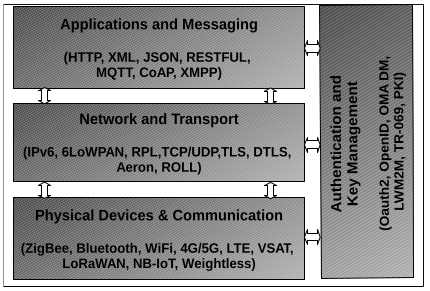
\includegraphics[scale=0.60]{figures/iot/iot_standards_protocols.png}}
	\caption{Source: \cite{khan_iot_2018} - Common IoT standards and protocols}
	\label{fig}
\end{figure}

As for every other connected device, IoT objects need to be uniquely identified on the network. For this purpose, nodes are usually identified by the mean of their MAC address and IP address. This mechanism leaves the network exposed to low-level Sybil and Spoofing attacks. This attack can be conducted by malicious Sybil nodes and may lead to serious resource scarcity, in an environment which is basically resource-constrained. Current object identification and locating mechanisms in IoT in general are exposed to a large number of vulnerabilities and operational attacks, making it a very active research topic \cite{zhang_iot_2014}.

The combination IPv6/Bluetooth is also as vulnerable as commonly used in WSNs. IEEE 802.15 standard requires fragmentation for IPv6 packets. Malicious nodes capacity to capture fragments and replay their duplicates may cause some security issues such as energy drainage or buffer overflows. This attack is known as fragmentation replay and duplication attack. IPv6 routing protocol  is also susceptible to some attacks when combined with the Routing Protocol for Low-Power and Lossy Networks, known as RPL routing attacks. It’s even more important to consider Ipv6 security, as Ipv4 won’t be able to accommodate all connected devices on the long term with their exponential number increase.

These network standards are subject to several network attacks such as session establishment and resumption attack. This consists in forging messages in order to hijack a session. In this scenario, a malicious node can spoof another legitimate node’s identity and act as a proxy between it and its counter part communicating node. In a word, weak security measures in the network will facilitate MITM-based attacks.

In addition to network related vulnerabilities, IoT objects can also present serious system issues, whether on the physical or the OS level.

%[TODO: add relevant bibliographies to previous paragraphs from [7]’s bibliography]

Appendix~\ref{app:wifi_attack} is a snippet on how vulnerable some of the commonly used network standards in Wireless Sensor Networks (WSNs) can be.

\subsection{Real-context risks \& mitigation}

A fact which stands out when looking closer at the IoT security industry, is the huge gap between the adoption of IoT for business and the adoption of IoT security practices. We require IoT security by design to ensure life-cycle sustainability for IoT devices \cite{thales2}.
When looking at different IoT solutions developed in the industry, we first look at common issues and vulnerabilities as a starting nail to track corresponding solution products. OWASP IoT Top 10 \cite{owasp-iot-10} nicely  summed up these vulnerabilities, giving an outer view of the threat landscape. In a addition to new and upcoming regulations, these issues make the conducting vectors driving the IoT security industry. No wonder they are mostly technical based, since the very purpose of developing a security technology is to hunt some specific threat.

\subsubsection{Default passwords}

A first approach to solve the problem is to look at how this password hard-coding is realized, and so, work the process straight out. The first point is that these passwords are too weak. Using a wordlist of common IoT devices passwords, an attacker is able to carry out a dictionary-based attack and take over the device. So was the case of Mirai alike attacks as explained above. The second point concerns the use of that same password all along the devices life-cycle. Users never bother to change them, assuming they are fully aware that their device can be remotely accessed using that password. Third point is that these passwords are hard-coded, so they can be quickly retrieved with old fashion reverse engineering. Moreover, they are usually stored in plain text or in a weak hash scheme, such as MD5, in order to save computing power.

The first point can fixed by requiring secure default password policies, including password length, complexity and uniqueness. Second point could be solved using password expiration and one-time password. The latter will force users to change default passwords when setting up their IoT infrastructure. Once again, we assume here that users have been notified of their device using a password in the first place. The third point is a bit more challenging to spear. As mentioned, it comes a consequence of the power-constraint nature of IoT devices. Hence, it’s difficult to work it out, without wrecking the device’s performance.

An alternative approach to address this issue is to sum up several authentication layers. Passwords is actually an authentication mechanism among others. Therefore, adding extra authentication can mitigate the risk of password compromise. This can be implemented through two-factor authentication, bio-metric authentication, Single Sign On tokens (SSO), digital certificates and PKI. 

It’s vital to bear in mind that this password issue is basically authentication related. Whereas authentication can be realized throughout who we are, what we know and what we possess. From this perspective, passwords is something we know. If it burdens vulnerabilities, we can just bypass it by exploring other information we know, alongside who we are and what we possess. An IoT devices fleet is usually relatively widespread geographically, making the  latter two authentication strategies merely feasible.

\paragraph{Solutions}

\begin{itemize}
	\item One-time passwords (OTP)
	\item Temporary one-time passwords (TOTP)
	\item Smart card based SSO
	\item eSIM
\end{itemize}

%One-time passwords (OTP)\\
%Temporary one-time passwords (TOTP)\\
%Smart card based SSO\\
%eSIM

\subsubsection{Irregular patches and updates}

Once the IoT infrastructure is set up, the device fleet remains mostly static, and that can lead to tremendous disasters. Devices come with embedded firmware. And like almost any firmware, it can be reverse engineered and pwned. Overtime, a firmware is susceptible to become obsolete and vulnerable. That’s why patches and upgrades are vital against common security vulnerabilities and 0-Days exploits.

The Satori attack is a good example to illustrate the risk \cite{arstechnica}. The attack occurred when hackers exploited critical vulnerabilities in wide range of routers (D-Link, Huawei, RealTek ...), allowing them to get a RCE, in order to build up large IoT botnets. These botnets were exploited at first to conduct massive DDoS attacks, and later on, to mine digital coins. Besides, Satori’s payload include a worm to allow the infection of neighboring devices with no human interaction needed, in a Stuxnet fashion.

The problem with upgrading IoT devices resides in the fact that these are usually widespread out there in the field. It’s difficult to deliver an update to a thermo-sensor deployed in a farm for instance. Some solutions exist though, even if they only solve the problem partially.

\paragraph{Solutions}

\begin{itemize}
	\item Pre-signed URL
\end{itemize}

%Pre-signed URL

\subsubsection{Insecure interfaces}

IoT devices aren’t standalone components. They implement network protocols for communication (e.g. Bluetooth, LPWAN ...), services for maintenance (e.g. Telnet) and applications for data processing and storage. These interfaces comes with their own vulnerabilities, whether generic or specific to the IoT implementation. Thus, they increase the attack surface.

The main strategy for mitigating this risk available right now is encryption. This particularly involves the use of digital certificates (e.g. X509). The ENISA report on “Good Practices for Security of IoT” \cite{enisa} highlights above all security by design. Security has to be bared in mind all along the device’s design and implementation, from the very cradle to the grave. The Best Practices to mitigate interface related risk involve application of ENISA good practices related to used standards. In other terms, one must apply security measures not only limited to the device itself, but take a step further to pack in the entire ecosystem and bring it under control.

\paragraph{Solutions}

\begin{itemize}
	\item Thales Trusted Key Manager
	\item Remote subscription management
	\item IQNOX IAM platform
\end{itemize}

%Thales Trusted Key Manager\\
%Remote subscription management\\
%IQNOX IAM platform

\subsubsection{Data exposure}

Smart devices are specifically designed to carry out tasks where they handle large amount of data. A common risk in IoT security is data leakage. Scandals and large-scale attacks made lack of data protection in the IoT a top concern in the industry. Whether stored data at rest or active data being exchanged, it has to be safe from unauthorized access.

All communications at all layers have to be secured, how insignificant the layer might seem. An attack on a casino reported by Darktrace in 2017 demonstrates how expensive insufficient data protection can be \cite{thesun}. The attackers in this case actually exploited lack of communications security in a smart thermometer of an aquarium exposed in a casino. They used this smart device to get a foothold in the casino’s network, then going up to the cloud, and finally exfiltrate 10Gb of the casino’s customers stored data.

The most efficient way at disposal to address this threat is cryptography. It defends against data theft for stored data and eavesdropping for over-the-network data. It preserves therefore the data privacy, integrity and confidentiality. Data at rest must, besides its encryption, be stored on an under-control host. When communicating, a secure channel with the counterpart shall be established and messages exchanged should be encrypted (confidentiality) and signed (integrity). Looking up to the previously described attack, we first notice the unencrypted communications which allowed the attackers to get their foothold in the first place. And second, the data were insecurely stored, which allowed the hackers to quickly fetch the database files and exfiltrate them.

\paragraph{Solutions}

\begin{itemize}
	\item Thales embedded Secure Element (eSE)
	\item Trusted Platform Module (TPM)
\end{itemize}

%Thales embedded Secure Element (eSE)\\
%Trusted Platform Module (TPM)

\subsubsection{IoT fleet management}

With the increase of connected IoT devices and the sophistication of its inter connection, the risk of misuse or mismanagement of some increases as well. A more and more common issue consist in IT teams not aware of what and how many connected devices they have inside their their network \cite{helpnetsecurity}. Within the same line, we are facing a rising number of “Shadow IoT and IoMT devices”. Among the most dangerous discoveries, one concerns the use of Facebook and YouTube applications of medical devices operating Windows XP. Having a medical device connected running insecure web applications on an obsolete and unsupported OS is not only a cyber threat, but a threat to human life. This kind of mismanagement made such schemes a beloved target for ransomware attacks \cite{cpomagazine}.

Therefore, it’s crucial to deploy IoT management platform whenever it’s necessary. IoT management platforms facilitates the monitoring of different devices connected to its network. It can be seen as an inventory of objects, which provides information about their status, connectivity, access logs, running apps and services ... etc. With such a global overview, one can set up security counter measures much easier, because this kind of information flow can easily fit in as an input for a SIEM or an IDS/IPS in order to automatically spot among others paranormal behavior, unusual access, collusion between subnets or VLANs, and foremost, shadow IoT devices. Obsolete or vulnerable devices can then be upgraded or patched. Improper network segmentation can be fixed. Shadow devices shall be disposed of.

\paragraph{Solutions}

\begin{itemize}
	\item Azure IoT management platform
	\item IBM IoT management platform
\end{itemize}

%Azure IoT management platform\\
%IBM IoT management platform

\subsection{Legal framework evolution}

Another vector driving the IoT security industry is the evolution of national and international regulations. Companies have to adapt their technical standards to meet requirements of laws which recently came into force. The EU voted the Cybersecurity Act in 2019, which already sets standards for IoT security manufacturers. The law was pushed by ENISA in order to curb IoT related risks. The US followed the trend with the IoT Cybersecurity Improvement Act late 2020. A bill passed on by British regulators require IoT devices sold in the UK to embed a “reasonable security feature”.